\section{Mutation Operators}
\label{sec:mutation}
Mutation is one of the most important operators of genetic algorithms. It prevents the algorithm from getting stuck in a local minimum. It adds randomness in the evolutionary process and can help to find genes, which were lost and cannot be reproduced otherwise. In other words, mutation diversifies the population.\par
Mutation operators for the TSP make random permutations of the cities and they can therefore modify the tour to a large degree. The mutation operators which are discussed below will be applied only to the path representation. Applying them on the adjacency representation can ruin the tour. For instance, let us consider the following tour in the path representation 01432 which corresponds to the tour 14023 in the adjacency representation. If we swap two cities 1 and 3, it results in the tour 03412 in the path representation. The Hamilton cycle is still there. If we also swap the entries 1 and 3 in the adjacency representation, we get 34021. The corresponding graph in Figure \ref{mut_intro} illustrates that there exist two cycles and the Hamilton cycle was destroyed. \par

\begin{figure}[htp] \centering
	\centering
	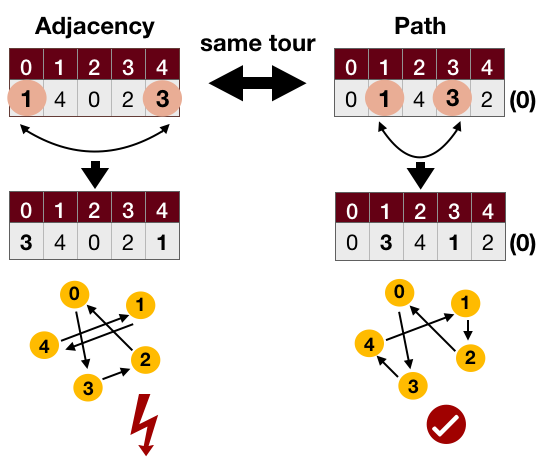
\includegraphics[width=0.4\textwidth]{Mut_Intro}
	\caption{Swapping cities in adjacency and path representation.}
	\label{mut_intro}
\end{figure}

The \textbf{Swap mutation} operator as discussed by \citeauthor{potvin1996genetic} \cite{potvin1996genetic} modifies the tour slightly, only exchanging the positions between two cities. Given the chromosome 014532 the swap mutation between the cities 1 and 3 which occupy the positions 1 and 4, respectively, transforms the chromosome into 034512 (see Figure \ref{swap_mutation}).

\begin{figure}[htp] \centering
	\centering
	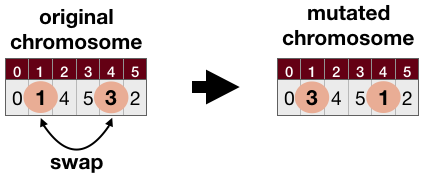
\includegraphics[width=0.4\textwidth]{swap_mutation}
	\caption{Swap mutation for the chromosome 014532 when swapping the cities 1 and 3.}
	\label{swap_mutation}
\end{figure}


The \textbf{Scramble mutation} operator as discussed by \citeauthor{potvin1996genetic} \cite{potvin1996genetic} takes two indices, which define two cut points. The cities between these cut points are randomly permuted. Given the chromosome 014532, the scramble mutation for the cut points 1 and 4 can generate, for instance, the chromosome 035142 (see Figure \ref{scramble_mutation}).

\begin{figure}[htp] \centering
	\centering
	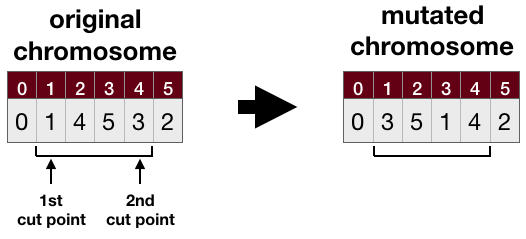
\includegraphics[width=0.4\textwidth]{scramble_mutation}
	\caption{Scramble mutation for the chromosome 014532 with the cut points 1 and 4.}
	\label{scramble_mutation}
\end{figure}


The \textbf{Shift mutation} operator as used by \citeauthor{akay2013recent} \cite{akay2013recent} has two random components: a random city and a random integer. The chosen city will be shifted to the left or to the right, depending which shift is used. The chosen integer corresponds to the number of positions by which the chosen city will be shifted. Given the chromosome 014532, let us assume that the random city is the city 1 and the random integer is 3. We will use the right shift. Therefore, the city 1 will be shifted to the right by 3 positions (see Figure \ref{shift_mutation}).

\begin{figure}[htp] \centering
	\centering
	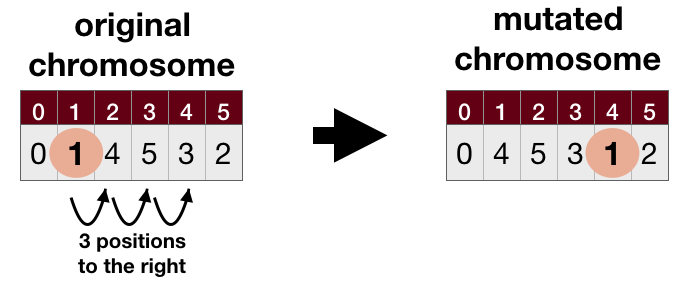
\includegraphics[width=0.4\textwidth]{shift_mutation}
	\caption{Right shift mutation for the chromosome 014532 with random city 1 and random integer 3.}
	\label{shift_mutation}
\end{figure}

If the chosen integer is greater than the number of remaining steps to the right (or to the left, if the left shift is chosen), then the shift continues at the beginning of the chromosome. For instance, if the random integer was 5 in the example above, then the city 1 will be at the position 0 (see Figure \ref{shift_mutation_torus}).

\begin{figure}[htp] \centering
	\centering
	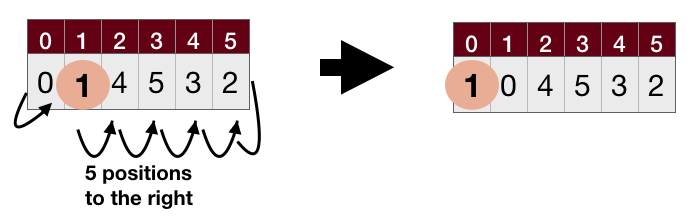
\includegraphics[width=0.4\textwidth]{shift_mutation_torus}
	\caption{Right shift mutation for the chromosome 014532 with random city 1 and random integer 5.}
	\label{shift_mutation_torus}
\end{figure}


The \textbf{Inversion mutation} operator as used by \citeauthor{akay2013recent} \cite{akay2013recent} takes two indices which define two cut points. The order of the cities between them is inverted. Given the chromosome 014532, the inversion mutation for the cut points 1 and 4 generates the chromosome 035412 (see Figure \ref{inversion_mutation}).

\begin{figure}[htp] \centering
	\centering
	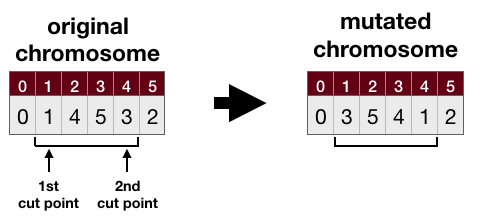
\includegraphics[width=0.4\textwidth]{inversion_mutation}
	\caption{Inversion mutation for the chromosome 014532 and cut points 1 and 4.}
	\label{inversion_mutation}
\end{figure}

The \textbf{Insertion mutation} operator as used by \citeauthor{akay2013recent} \cite{akay2013recent} takes two indices, which define two cut points. The cities which occupy the positions between the first cut point (exclusively) and the second cut point (inclusively) are shifted one position to the left. The city which occupied the index, which corresponds to the first cut point, now goes at the index, which corresponds to the second cut point, i.e. this stands after the set of shifted cities now. Given the chromosome 014532, the insertion mutation for the cut points 1 and 4 generates the chromosome 045312 (see Figure \ref{insertion_mutation}).

\begin{figure}[htp] \centering
	\centering
	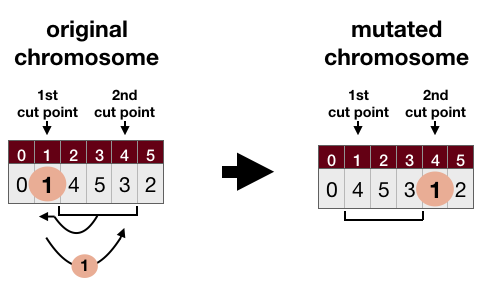
\includegraphics[width=0.4\textwidth]{insertion_mutation}
	\caption{Insertion mutation for the chromosome 014532 and cut points 1 and 4.}
	\label{insertion_mutation}
\end{figure}

The \textbf{Displacement mutation} operator \cite{akay2013recent} takes three indices, which define three cut points. The cities which occupy the positions between the first cut point (inclusively) and the second cut point (inclusively) are shifted at the position after the third cut point.  This means that the cities between the second cut point (exclusively) and the third cut point (inclusively) are moved to the left, where the first cut point was. Given the chromosome 01453276 the displacement mutation for the cut points 1, 4 and 6 generates the chromosome 02714536 (see Figure \ref{displacement_mutation}).

\begin{figure}[htp] \centering
	\centering
	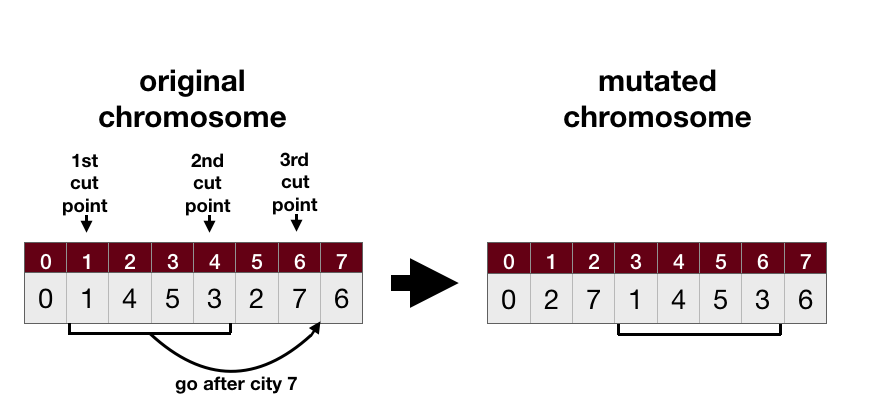
\includegraphics[width=0.5\textwidth]{displacement_mutation}
	\caption{Displacement mutation procedure for the chromosome 01453276 and cut points 1, 4, and 6.}
	\label{displacement_mutation}
\end{figure}